\section{Token-Budget Comparisons with WSD}
\label{sec:app-river}

In \Cref{fig:pretrain} (right) and \Cref{fig:bema_sf} (right) we compared
\pace\ at a constant learning rate to AdamW with linear decay to zero. In this
appendix we make that comparison systematic for pretraining and interpret both
regimes. The analysis is inspired by the token-budget comparisons used to
study Schedule-Free methods \citep{defazio2024schedule,song2025river}, and we
read it through the river-valley description of the loss landscape
\citep{wen2024warmup,song2025river}: at a constant learning rate, the iterate
oscillates along the steep ``hill'' directions of a valley while making steady
progress along its flat ``river'' floor, and the decay phase of WSD acts by
suppressing this oscillation and bringing the iterate down to the floor. This
perspective makes clear both the appeal of WSD and its cost: although the
decay phase produces the characteristic sharp drop in loss at the end of
training, until it begins the loss curve overstates the loss the model could
achieve, so that model quality is difficult to assess mid-training, and once
it begins, the remainder of the run is committed to a single token budget. An
optimizer whose returned iterate already lies on the river floor incurs
neither cost: its loss curve reflects post-decay performance at every step of
training, and training may be stopped or continued at any point.

The token-budget comparison tests exactly this property. Because a decay
branch primarily removes oscillation while making little further progress
along the river, the endpoint of a branch launched at a given budget estimates
the position of the river at that budget. Comparing the endpoints of branches
launched at several budgets to a candidate trajectory thus determines whether
that trajectory tracks the river: endpoints that coincide with the trajectory
indicate that it already lies on the floor, while endpoints that fall below it
reveal residual oscillation that a decay phase would have removed. We run
this comparison in both regimes---branches at $50\%/75\%/100\%$ of the
pretraining budget, and at three budgets and two learning rates in
fine-tuning---with all runs sharing data, batch size, and base learning rate.

\paragraph{Pretraining.}
In \Cref{fig:appendix_pretrain_river}, we overlay the AdamW decay branches on
the \pace\ constant-learning-rate trajectory. Every branch lands on the
trajectory: the endpoints ($3.721/3.597/3.530$) match \pace\ at the same budgets
($\approx 3.707/3.595/3.534$) to within $0.014$, and to within $0.004$ at the
full budget---closer than the seed-to-seed spread. At every budget, decaying the
learning rate only recovers the loss that \pace\ already reaches without a
schedule.

\begin{figure}[t]
  \centering
  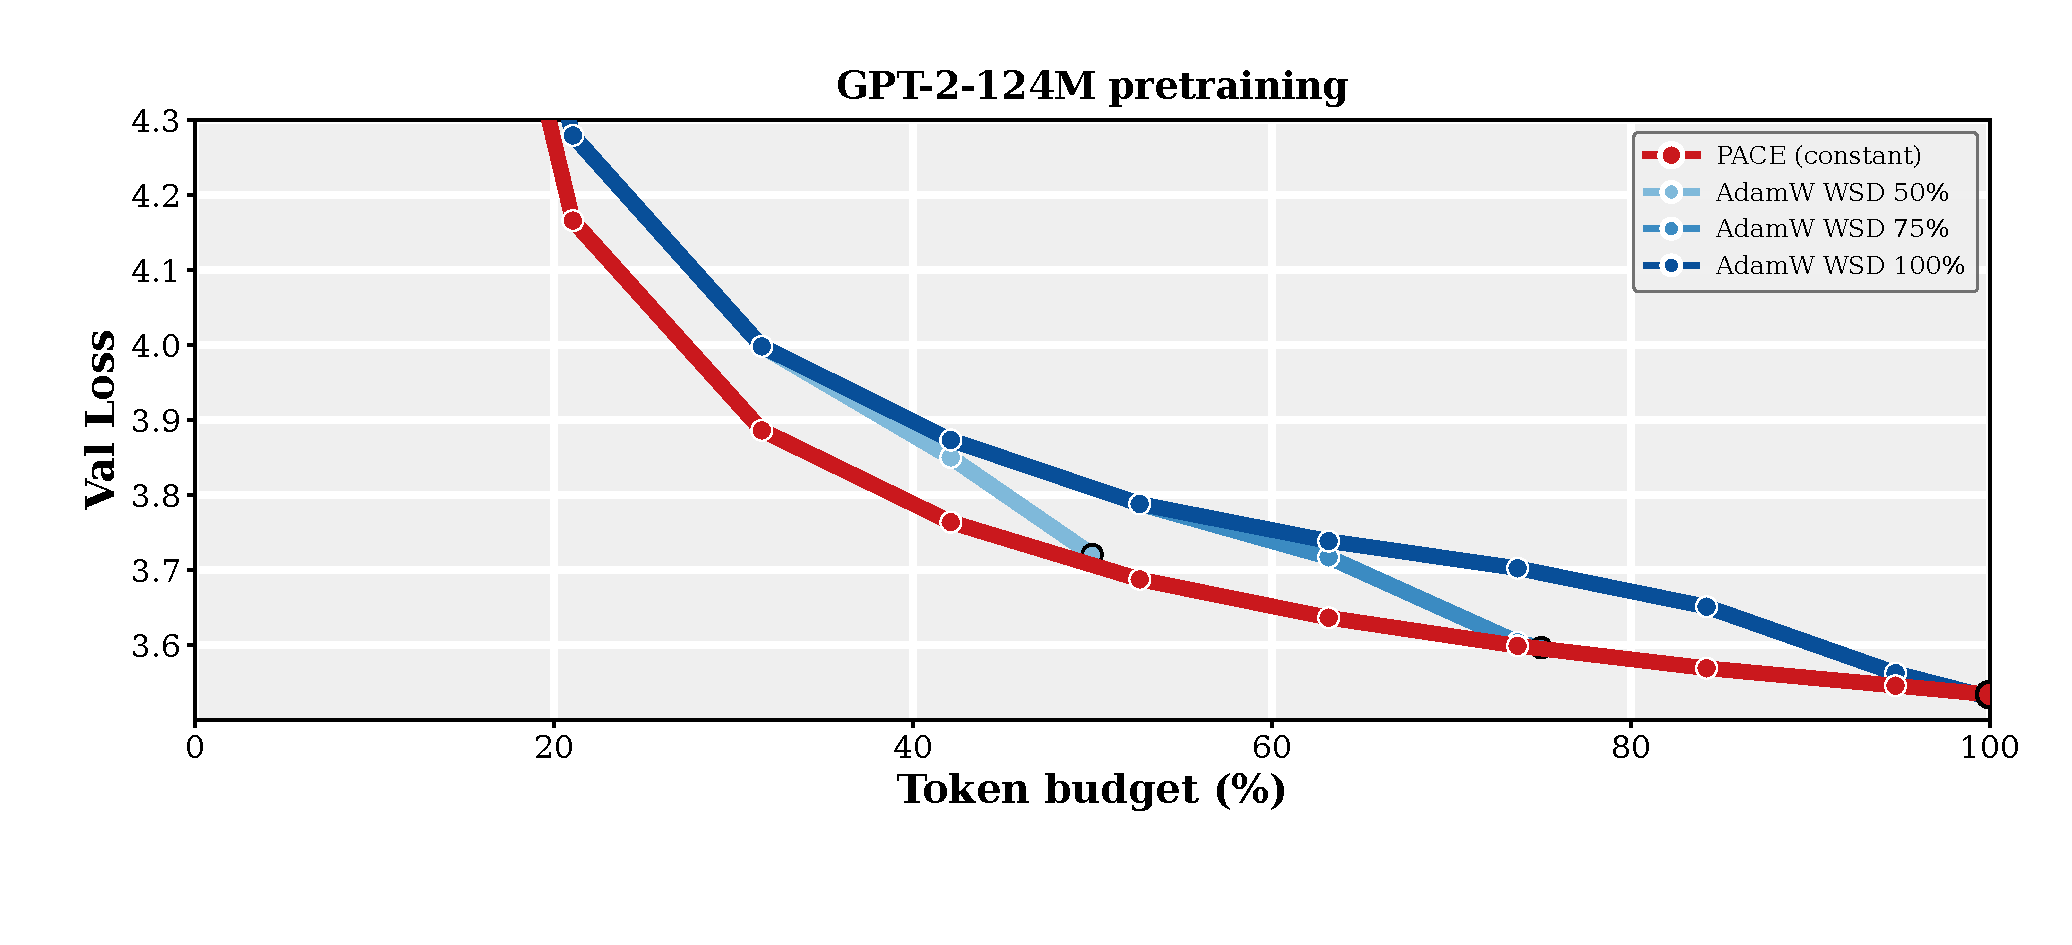
\includegraphics[width=0.676\textwidth]{figures/fig_appendix_pretrain_river.pdf}
  \caption{\textbf{Token-budget comparison on GPT-2-124M pretraining.}
  AdamW WSD decay branches at $50\%/75\%/100\%$ of the token budget overlaid on
  the \pace\ constant-learning-rate trajectory; each branch endpoint lands on
  the \pace\ trajectory, so the decay phase only recovers the loss that \pace\
  attains continuously without a schedule.}
  \label{fig:appendix_pretrain_river}
\end{figure}

\paragraph{Fine-tuning.}
The fine-tuning comparison in \Cref{fig:bema_sf} (right) yields a stronger
conclusion: every budget-matched branch ends above the \pace\ trajectory, with
endpoints of $1.277/1.233/1.205$ against \pace\ at $1.153$, and the gap widens
at larger learning rates. In this regime, no decay branch reaches the loss of
the constant-learning-rate \pace\ run at any budget.

\paragraph{Peeling off intermediate checkpoints to decay.}
Across every budget, learning rate, and regime that we tested, no decay
branch ends below the \pace\ trajectory, which is precisely the behavior this
comparison associates with a trajectory that already lies on the river floor.
The practical consequences are those identified above: the validation curve
of \pace\ reflects post-decay performance at every step, so that model
quality is visible throughout training, and the loss that WSD attains only at
the designated endpoint of a branch is available at every budget, without
fixing a training horizon in advance. In fine-tuning, we find the stronger
conclusion that the \pace\ trajectory lies below every budget-matched branch
endpoint, suggesting that the modified trajectory makes faster progress along
the river than the trajectory from which the branches descend.

